\section{Propietats de les sèries temporals}

\todo{}
 (Trets semàntics/patologies/representacions(tipus/funció temporal))



\subsection{Trets semàntics de les sèries temporals}

Una sèrie temporal pot provenir d'àmbits varis i per tant tenir un
significat variat. És el que anomenem trets semàntics de les sèries
temporals.


En el model d'operacions s'ha vist que l'atribut de temps de les
sèries temporals indueix vàries naturaleses en el comportament dels
operadors: com a conjunts, com a seqüències o com a funcions
temporals. Però aquesta distinció de significat és des del punt de
vista de formalització matemàtica per l'estructura de les sèries
temporals.

A continuació distingim el significat de les sèries temporals segons
l'origen; és a dir com s'han adquirit o de quin entorn
provenen. Aquesta distinció és important per a determinar quines
operacions tenen sentit de ser aplicades i quines no a una sèrie
temporal en particular. Així \textcite{segev87:sigmod} anomena
comportament semàntic (\emph{semantic behavior}) a la varietat de
formes que pot prendre una sèrie temporal segons l'àmbit on
s'apliquen.



Classifiquem els trets semàntics a grosso modo
\todo{}


Un primer tret semàntic de les sèries temporals és deu al mètode
d'adquisició. Així una sèrie temporal es pot classificar segons si
s'ha adquirit mostrejant un senyal continu cada cert període o si
prové d'una acumulació o d'un comptatge d'esdeveniments en un cert
període de temps. Aquests són els dos orígens principals que poden
tenir els senyals discrets segons
\textcite[cap.~1]{proakismanolakis96}.  En aquest tret es distingeix
segons l'adquisició en l'eix del temps, també es pot distingir segons
si l'adquisició en l'eix de valors és contínua o discreta però això és
un tret propi dels valors i, com a característica, pertany al domini
dels valors. Aquest procés en l'eix de valors s'anomena quantització
del senyal però sovint, per simplificar, no es té en
compte \parencite{proakismanolakis96}.%S1.4.7




 \todo{però aquí no volem parlar d'adquisició sinó de
  naturalesa: magnituds i comptadors} 

Així doncs segons el mètode d'adquisició, classifiquem una sèrie
temporal amb trets de magnitud o de comptador. Aquest tret
semàntic cal tenir-lo en compte ja que quan s'adquireix una magnitud
es veu el seu estat instantani actual, mentre que quan s'adquireix un
comptador ofereix informació de la seva variació respecte a
l'adquisició anterior. 

Els comptadors poden oferir la informació de diverses formes: en valor
absolut, en valor relatiu i en velocitat. 


Mesures vs increments d'un comptador vs gràfics barres (eix y: freqüència) i histograma (eix y: densitat de freqüència) \autoref{fig:model:comptador-formes}

$S_m = \{(0,0),(2,1),(4,3),(5,4),(9,10)\}$

$S_\Delta = \glssymbol{not:sgst:gradient}(S_m) = \{(0,0),(2,1),(4,2),(5,1),(9,6)\}$

$S_v = S_\Delta / \glssymbol{not:sgst:gradient}(S_m map(t,t)) =
\glssymbol{not:sgst:gradient}(S_m) = \{(0,0),(2,0{,}5),(4,1),(5,1),(9,2)\}$ \todo{faltar definir la funcio map (t,v)->(t,t), dir-ne funció temps?}


\begin{figure}[tp]
  \centering
    \begin{subfigure}{\textwidth}
    \centering
  \begin{tabular}[c]{|c|c|}
    \multicolumn{2}{c}{$S_a$} \\ \hline
    $t$  & $v$ \\ \hline
    0   & 0 \\
    2   & 1 \\
    4   & 3 \\
    5   & 4 \\
    8   & 10 \\ \hline
  \end{tabular} \qquad
  \begin{tabular}[c]{|c|c|}
    \multicolumn{2}{c}{$S_\Delta$} \\ \hline
    $t$  & $v$ \\ \hline
    0   & 0 \\
    2 & 1 \\
    4 & 2 \\
    5 & 1 \\
    8 & 6 \\ \hline
  \end{tabular} \qquad
  \begin{tabular}[c]{|c|c|}
    \multicolumn{2}{c}{$S_v$} \\ \hline
    $t$  & $v$ \\ \hline
    0   & 0 \\
    2 & 0{,}5 \\
    4 & 1 \\
    5 & 1 \\
    8 & 2 \\ \hline
  \end{tabular}
  \caption{Taules de valors}
  \end{subfigure}

  \begin{subfigure}{0.3\textwidth}
  \begin{tikzpicture}
    \begin{axis}[
        timeseriesrel,
        title=$S_a$,
        ]
    \addplot[blue] coordinates {
        (0,0)
        (2,1)
        (4,3)
        (5,4)
        (8,10)
    };
    %\addlegendentry{Valor absolut}
    \addplot[only marks,mark=*,red] coordinates {
        (0,0)
        (2,1)
        (4,3)
        (5,4)
        (8,10)
    };
    % \addlegendentry{Punts de mesura}
    \end{axis}
  \end{tikzpicture}
  \caption{Valor absolut}
    \label{fig:model:comptador-formes:absolut}
  \end{subfigure}
  \begin{subfigure}{0.3\textwidth}
  \begin{tikzpicture}
    \begin{axis}[
        timeseriesrel,
        title=$S_\Delta$,
        ]
    \addplot[ycomb,blue,mark=-] coordinates {
        (0,0)
        (2,1)
        (4,2)
        (5,1)
        (8,6)
    };
    %\addlegendentry{Increments}
    \addplot[only marks,mark=*,red] coordinates {
        (0,0)
        (2,1)
        (4,2)
        (5,1)
        (8,6)
    };
    %\addlegendentry{Punts de mesura}

    \addplot[gray,dashed] coordinates {
        (0,0)
        (2,1)
        (4,2)
        (5,1)
        (8,6)
    };
    % \addlegendentry{Tendència}

    \end{axis}
  \end{tikzpicture}
  \caption{Increments}
  \label{fig:model:comptador-formes:increments}
  \end{subfigure}
 \begin{subfigure}{0.3\textwidth}
  \centering
  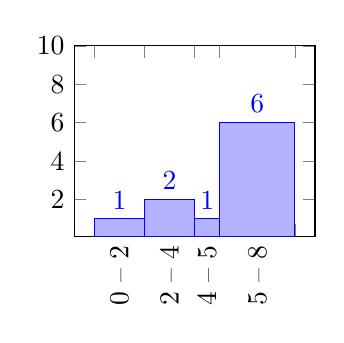
\begin{tikzpicture}
    \begin{axis}[
%        timeseriesrel,
        height=4cm,
        %width=10cm,scale only axis, height=5cm,
        ymax = 10,
        xtick = data,
        xticklabel interval boundaries,
        x tick label style= {rotate=90,anchor=east},
        x label style ={ at={(1,0)},left,yshift=0pt},
        ]
    \addplot[ybar interval,blue,fill=blue!30!white] coordinates{
        (0,1)
        (2,2)
        (4,1)
        (5,6)
        (8,6)
    }; 
    % \addlegendentry{Increments}

    \node[color=blue,above] at (axis cs:1,1) {1};
    \node[color=blue,above] at (axis cs:3,2) {2};
    \node[color=blue,above] at (axis cs:4.5,1) {1};
    \node[color=blue,above] at (axis cs:6.5,6) {6};
    \end{axis}
  \end{tikzpicture}
  \caption{Gràfic de barres}
    \label{fig:model:comptador-formes:barres}
  \end{subfigure}

  \begin{subfigure}{0.3\textwidth}
  \centering
  \begin{tikzpicture}
    \begin{axis}[
        timeseriesrel,
        title=$S_\Delta$
        ]
    \addplot[blue] coordinates {
        (0,0)
        (2,1)
        (2,0)
        (4,2)
        (4,0)
        (5,1)
        (5,0)
        (8,6)
        (8,0)
    };
    %\addlegendentry{Valor relatiu}
    \addplot[only marks,mark=*,red] coordinates {
        (0,0)
        (2,1)
        (4,2)
        (5,1)
        (8,6)
    };
    %\addlegendentry{Punts de mesura}
    \end{axis}
  \end{tikzpicture}
  \caption{Valor relatiu}
    \label{fig:model:comptador-formes:relatiu}
  \end{subfigure}
  \begin{subfigure}{0.3\textwidth}
  \centering
  \begin{tikzpicture}
    \begin{axis}[
        timeseriesrel,
        title=$S_v$,
        ymax=2.3,
        ]
    \addplot[const plot mark right,blue] coordinates {
        (0,0)
        (2,0.5)
        (4,1)
        (5,1)
        (8,2)
    };
    %\addlegendentry{Velocitat mitjana}

   \addplot[only marks,mark=*,red] coordinates {
        (0,0)
        (2,0.5)
        (4,1)
        (5,1)
        (8,2)
    };
    %\addlegendentry{Punts de mesura}

    \end{axis}
  \end{tikzpicture}
  \caption{Velocitat}
    \label{fig:model:comptador-formes:velocitat}
   \end{subfigure}
  \begin{subfigure}{0.3\textwidth}
  \centering
  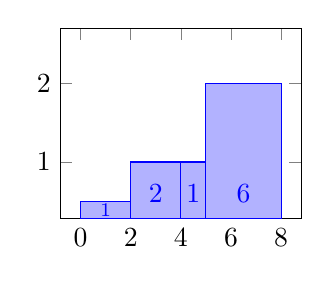
\begin{tikzpicture}
    \begin{axis}[
        height=4cm,
        ymax=2.7,
        ]
    \addplot[ybar interval,blue,fill=blue!30!white,mark=none] coordinates {
        (0,0.5)
        (2,1)
        (4,1)
        (5,2)
        (8,2)
    };
    %\addlegendentry{distribució d'increments}

    \node[color=blue] at (axis cs:1,0.39) {\scriptsize 1};
    \node[color=blue] at (axis cs:3,0.6) {2};
    \node[color=blue] at (axis cs:4.5,0.6) {1};
    \node[color=blue] at (axis cs:6.5,0.6) {6};
     \end{axis}
  \end{tikzpicture}
  \caption{Histograma}
  \label{fig:model:comptador-formes:histograma}
  \end{subfigure}

  \caption{Formes d'un comptador monòton}
  \label{fig:model:comptador-formes}
\end{figure}




\todo{explicar que d'una magnitud també es poden calcular els increments, etc. peo això no vol dir que siguin comptadors perquè no sabme què ha passat entremig}
i al revés tampoc: podem tenir un comptador però no recuperar-ne la magnitud (els valors instantanis) 

Els comptadors tenen fons d'escala, per tant l'eix de valors és circular

Els comptadors físics normalment són digitals però no té perquè ser així





* comptadors -> conservar totals (comptador: monòton, doble, relatiu)
usualment són digitals en naturalesa (compten amb naturals) però també poden ser analògics (comptar amb reals, per exemple comptar el cabal d'aigua, l'energia consumida, etc.).






\begin{example}
  
Un exemple de sèrie temporal amb tret de magnitud és la potència
instantània elèctrica i un exemple de comptador és la quantitat
d'energia elèctrica.

Exemple amb energia elèctrica:  

* magnitud: potència instantània
* comptador valor absolut: energia 
* comptador d'increments/valor relatiu/gràfic de barres: energia amb reset a cada lectura
* comptador de velocitat/histograma: potència mitjana

\end{example}







segons adquisició:

* contínua
* discreta (en base a clock?)






El valor d’una magnitud física es pot calcular com el producte d’un valor nu-
mèric per una unitat:
magnitud física = valor numèric x unitat [llibreverd IEC-IUPAC]



segons timestamp vs time span:

* timestamp: el típic de sèries temporals
* time span: 
- ex. $S=\{(gen,1),(feb,4),(mar,0)\}$: això són sèries temporals? o són dades intervals temporals? Es poden expressar/entendre com a sèries temporals via timestamps amb granularitat? Es poden expressar/entendre com a sèries temporals via tractar-les com a compadors?  
- també cal pensar en les sèries temporals de tipus temperatures mitjanes dels mesos d'octubre  $S=\{(oct98,1),(oct99,4),(oct00,0)\}$. Això com encaixa amb el nostre model de sèries temporals? això sí que s'anomenen sèries temporals, tot i que els escau molt bé la definició de seqüències temporals, i s'hi apliquen mètodes d'anàlisi de sèries temporals
- altre ex. cas d'una partitura musical  $S=\{(1,do),(2,re),(4,silenci),(5,fa),(7,silenci)\}$  es pot descriure com una sèrie temporal conjuntament amb la respresentació ZOH però seria millor fer servir el model d'intervals temporals... $I=\{([1,2),do),([2,4),re),([5,7),fa)\}$






Perquè RRDtool diferencia entre comptadors i magnituds?









\subsection{Patologies de les sèries temporals}




\todo{?}

* Problemes en l'adquisició

* Problemes en el rellotge

* Valors estant limitats en un rang
En el nostra cas els valors estaran associats a una variable física, per tant seran conjunt finits i acotats, per tant podrem definir una cota inferior màxima (ínfim) i una cota màxima (suprem). Donat el conjunt de valors V, definim la conta mínima del conjunt com     (això ja ho tenies fet no!!!)

. El primer problema  és la gestió d’una quantitat enorme de dades.

El segon problema  es el de la necessitat de censurar les dades,  es a dir validar que les dades
siguin correctes i en cas contrari rebutjar-les o reconstruir-les.

El tercer problema es dóna quan el període de mostreig no  és regular,  és a dir que les dades no es recullen de manera uniforme en el temps, però les aplicacions no ho contemplen o volen treballar amb dades a intervals regulars, també anomenat dades equi-espaiades.

En el moment  de recol lecció de dades apareixen dos problemes: valors que en un instant de temps prefixat no s'han pogut recollir i valors que són falsos.



* Tractament/validació de dades

With reference to data validation, attribute interpolation functions
can cope with this process. When data has not been captured or has
been captured erroneously, it must be treated as unknown data.
\begin{itemize}
\item When data has not been captured it is unknown by nature. For
  example, we try to capture data from a sensor and there is no
  response.
\item When data is erroneously it must be marked as unknown. For
  example, we capture data from a sensor but it responses in a not
  reasonable time or we capture data that is clearly outside a
  reasonable limits.
\end{itemize}
As a consequence, attribute interpolation functions deals with these
two subprocesses: treating unknown data and marking data as
unknown. Following with real numbers, let unknown value be represented
by the improper element infinity ($\infty$).  



* dades desconegudes: mesura inexistent, temps de termini, límits (rang dels valors)


\subsubsection{Regularitat de les sèries temporals} 

Per a determinar la regularitat d'una sèrie temporal es defineix un
interval de temps $i_0=[t_I,t_I+\delta]$, a on $t_I$ és un instant de
temps i $\delta$ una durada de temps, i els seus intervals múltiples
$i_j=[t_I+j\delta\, ,\, t_I+(j+1)\delta]$ per
$j=0,1,2\ldots$. Aleshores, la regularitat de la sèrie temporal depèn
de la situació dels temps de les seves mesures en aquests intervals de
temps $i_j$.
 
Quan la situació temporal de les mesures prové del sistema
d'adquisició de dades aleshores cal notar que, en l'àmbit de
teoria del senyal, aquests intervals de temps s'anomenen intervals de
mostreig, $\delta$ s'anomena període de mostreig i $t_I$ s'anomena
temps inicial del mostreig.


Una sèrie temporal és regular quan les mesures són equidistants en el
temps, tal com ho anomenen \textcite{last:hetland}.  La regularitat
d'una sèrie temporal és crítica en algunes operacions perquè hi ha
algoritmes d'anàlisi de sèrie temporals que només es poden aplicar a
sèries temporals regulars.
\begin{definition}[Sèrie temporal regular]
  \label{def:st:regular}
  Sigui $S=\{m_0,\ldots,m_k\}$ una sèrie temporal, $t_I$ un instant de
  temps i $\delta$ una durada de temps, $S$ és regular si i
  només si $\forall m \in S(T(\min(S),\infty):T(m) - T(\ant(m)) =
  \delta$ a on definim $t_I=T(\min(S))$.
\end{definition}

Si una sèrie temporal és regular, l'anomenem sèrie temporal regular de
període de $\delta$ iniciada a $t_I$. Si el $t_I$ pot ser qualsevol
llavors simplement l'anomenem sèrie temporal regular de període
$\delta$.  Si notem l'àmbit de teoria del senyal, aquest període té
relació amb el període de mostreig.


Així doncs, per contraposició definim que una sèrie temporal és
\emph{no regular} o \emph{irregular} quan no és regular.  A
continuació distingim tres característiques que poden presentar les
sèries temporals no regulars: temps real, ultramostreig i inframostreig.

\todo{} L'adquisició de les mesures pot estar lligada a un sistema de
control de temps real, el qual sol ser el que mana sobre el temps atès
que les periodicitats del mostreig per a control són més elevades que
les del mostreig per als humans (aquests tenen un temps de resposta
més lent) \todo{citar el llibre de real time}.  El temps real causa
que tinguem sèries temporals no regulars però amb unes certes
característiques de periodicitat.  Així, seguint el vocabulari de
temps real, en les sèries temporals no regulars es poden distingir els
tres casos mencionats


Una sèrie temporal és de temps real quan a cada interval de mostreig
hi ha una i només una mesura. A més, l'interval de mostreig pot estar
fitar per una durada anomenada termini.
\begin{definition}[Sèrie temporal de temps real]
  \label{def:st:tempsreal}
  Sigui $S=\{m_0,\dotsc,m_k\}$ una sèrie temporal, $t_I$ un instant de
  temps, $\delta$ una durada de temps i $D$ una durada que indica
  termini, $S$ és de temps real si i només si $D\leq\delta$
  i $\forall n\in\{0,\ldots,|S|-1\}: |S[t_I+n\delta,t_I+n\delta+D)| = 1$. 
  % Altrament $\forall n\in\{0,\ldots,|S|-1\}: \exists!m \in
  % S[t_I+n\delta,t_I+n\delta+D)$
\end{definition}

Si una sèrie temporal és de temps real, l'anomenem sèrie temporal
mostrejada en temps real de període $\delta$ iniciada a $t_I$ i
compliment del termini $D$.  Si $D=\delta$, es pot anomenar que $S$ és
una sèrie temporal de temps real sense termini.

Pel que fa al temps inicial $t_I$, en el cas de les sèries temporals
de temps reals pot estar situat entre $T(\min(S))-\delta < t_I \leq
T(\min(S))$.  Així doncs, una sèrie temporal regular és també de temps
real. En el cas que una sèrie temporal compleixi els requeriments de
regular a excepció de $T(\min(S))=t_I$, és a dir de la qual les
mesures són equidistants però no té el temps inicial demanat,
aleshores només és una sèrie temporal de temps real.



Seguint en l'àmbit de temps real, quan no es compleix que a cada
interval de mostreig hi ha una i només una mesura pot succeir que hi
hagi un, o més d'un, interval amb cap mesura o amb més
d'una. Respectivament, ho anomenem interval inframostrejat i interval
ultramostrejat. 



Una sèrie temporal té intervals amb ultramostreig (\emph{upsampling})
quan en alguns intervals de mostreig hi ha una mesura o més d'una.
\begin{definition}[Sèrie temporal amb ultramostreig]
  Sigui $S=\{m_0,\dotsc,m_k\}$ una sèrie temporal, $t_I$ un instant de
  temps i $\delta$ una durada de temps, els intervals amb
  ultramostreig de $S$ són aquells que
  $|S[t_I+n\delta,t_I+(n+1)\delta)|>1$ a on $n\in\N$.
\end{definition}

Una sèrie temporal té intervals amb inframostreig
(\emph{downsampling}) quan en alguns intervals de mostreig no hi ha
cap mesura.
\begin{definition}[Sèrie temporal amb inframostreig]
  Sigui $S=\{m_0,\dotsc,m_k\}$ una sèrie temporal, $t_I$ un instant de
  temps i $\delta$ una durada de temps, els intervals amb
  inframostreig de $S$ són aquells que
  $|S[t_I+n\delta,t_I+(n+1)\delta)|=0$ a on $n\in\N$.
\end{definition}

Així doncs, una sèrie temporal no regular es pot classificar segons si
és de temps real i en el cas que no ho sigui es pot indicar si té
intervals amb ultramostreig o si en té amb inframostreig, sent aquests
dos darrers casos possibles alhora.





\subsubsection{Regularització de sèries temporals}

Com es regularitza una sèrie temporal amb els operadors de SGST? O com es canvia el període d'una sèrie temporal?

S'han d'utilitzar operadors de funció temporal. 

Així, com ja s'ha notat en les propietats del mateix operador, la
selecció temporal d'una sèrie temporal en un conjunt de temps
equi-espaiat $i = \{t_I+n\delta | n\in\mathbb{N}, n\leq s \}$ és una
sèrie temporal regular de període $\delta$ iniciada a $t_I$: $S[i]^r
\equiv \{ (t_I, v_0), (t_I+\delta,v_1), \dotsc , (t_I+s\delta,v_s)\}$
a on $r$ és una funció de representació.


Així doncs, la gràcia de regularitzar rau en la funció de representació.


\todo{descriure tècniques per regularitzar les de temps real, les d'inframostreig, les d'ultramostreig}

temps real: cas simple de regularització és aplicar representacions a trossos constants; si és de temps real es pot interpretar que en certa manera la mesura és vàlida per a tot l'interval.

ultramostreig: cas simple de regularització és agregar els intervals amb ultramostreig amb la mitjana, el màxim, etc.

inframostreig: cas simple es pot utilitzar el valor del següent o de l'anterior interval, és a dir també amb representacions a trossos constants. Aquest cas ja s'ha d'interpretat més aviat com una reconstrucció a diferència del temps real que interpretem com a vàlid.
\todo{el termini també podria ser relatiu entre mesures (temps de heartbeat)}
El termini $D$ descrit fins ara té relació amb el concepte de termini utilitza a temps real. També es poden utilitzar altres conceptes de termini com per exemple una fita del temps entre mesures. Això pot ampliar la validesa en el cas de l'inframostreig; és a dir si hi ha heartbeat més gran que el temps de mostreig vol dir que es permet l'inframostreig.



Més sobre això en els agregadors dels atributs del model de SGSTM que és on regularitzem sèries temporals...


\todo{potser es poden regularitzar fàcilment les de temps real,inframostreig i ultramostreig?}
es poden acceptar com a regulars, per exemple les de temps real es canvien els instants fent que siguin els del període de mostreig teòric, les d'ultramostreig se suprimeixin els punts ultramostrejats, els d'inframostreig es farceixen els forats ...

es plantegen com a planificació per a la posterior regularització; és a dir es planteja mostrejar una sèrie temporal a temps real i així després lligar-ho amb un mètode per a regularitzar-la.



\subsection{Graf i funció temporal de representació}
\label{sec:model:repr}
\todo{segev87 parla de tipus de la sèrie temporal}

Una sèrie temporal és la representació discreta d'una funció contínua;
la qual és una funció temporal atès que depèn del temps. El model de
SGST definit anteriorment formalitza la sèrie temporal com aquesta
representació discreta. Però a partir d'una sèrie temporal es pot
voler interpretar quina era la funció contínua original; és a dir
obtenir nous valors segons una funció a la que s'anomena graf d'una
funció (\emph{graph of a function}), en el sentit de gràfic
(\emph{plot}) que cal no confondre amb els grafs d'arestes i vèrtexs
(\emph{vertex-edge graph}).

\begin{definition}[Graf d'una sèrie temporal]%an. graph
  Sigui $S=\{m_0,\ldots,m_k\}$ una sèrie temporal i $T$ un domini del
  temps, es defineix el graf de la sèrie temporal
  $\glssymboldef{not:sgst:graf} S(t)$ com un conjunt de parells
  ordenats $(t,S(t)$ : $\glssymboldef{not:sgst:graf} S(t) = \{ (t,S(t)) |
  t\in T \}$ a on $S(t)$ és una funció de representació de la sèrie
  temporal.
\end{definition}

Per a calcular el graf d'una sèrie temporal es necessita una funció de
representació. Mentre que la funció que permet canviar d'una funció
contínua a una sèrie temporal s'anomena procés d'adquisició o
mostreig, la funció que permet canviar d'una sèrie temporal a una
funció contínua l'anomenem funció de representació.  Així doncs,
donada una sèrie temporal es poden definir funcions amb el temps com a
variable que calculin nous valors a partir de les mesures
emmagatzemades.
\begin{definition}[Funció de representació]
  Sigui $S=\{m_0,\ldots,m_k\}$ una sèrie temporal, es defineix $S(t)$
  com la funció de representació de la sèrie temporal contínuament al
  llarg del temps $t$; és a dir que per cada instant de temps la
  funció pren un valor: $\forall t\in T: v(t) = S(t)$. 

  Atenent a les operacions de càlcul que es facin per a obtenir $S(t)$
  diem que hi ha diverses funcions de representació. Així per a cada
  funció de representació indicarem a quina ens referim amb un
  superíndex \glsdispdef{not:sgst:frepr}{$S^r(t)$} a on
  \glssymboldef{not:sgst:repr} és el nom d'una funció de representació
  de la sèrie temporal.
\end{definition}

La utilitat de les funcions de representació és diversa i per això les
operacions de càlcul poden ser qualssevol. Una funció de representació
es pot utilitzar per a interpolar valors d'una sèrie temporal però
també per a extrapolar-los i fer prediccions o per a canviar la
resolució de la sèrie temporal. També es pot utilitzar per al problema
aproximar la sèrie temporal a la funció original; és a dir donar una
funció de representació que sigui la funció contínua que més
s'aproxima a la funció temporal original.


El lligam entre una sèrie temporal i la seva representació no és fix;
és a dir que donada una sèrie temporal es pot representar amb una
funció o amb una altra segons convingui.  Encara que en alguns àmbits,
per exemple a teoria del senyal o en algunes aplicacions de l'anàlisi
de sèries temporals, l'objectiu és cercar la parella de sèrie temporal
i representació que més s'aproxima a la funció contínua original; en
altres àmbits, com per exemple el del model multiresolució que definim
posteriorment, l'objectiu està més orientat a utilitzar
representacions de les sèries temporals segons els càlculs que es
volen fer o segons la naturalesa que s'assumeixi de la sèrie temporal.


No obstant, les funcions de representació s'han d'utilitzar amb
criteri. Per exemple la naturalesa de la sèrie temporal indueix a unes
possibles operacions de càlcul que es poden realitzar, per tant
l'aplicació de qualsevol funció de representació a la sèrie temporal
pot donar resultats incoherents. O bé un altre exemple és aplicar
càlculs successius a una sèrie temporal seguint diferents funcions de
representació.  

Així i tot, en la formalització del model de funcions de
representacions no hi definim cap criteri en concret per a, així,
donar llibertat en les possibilitats de càlcul amb les sèries
temporals. Al capítol \todo{ref} d'estat actual ja s'ha vist que en
l'anàlisi de sèries temporals hi ha diversitat en els algoritmes de
representació que s'utilitzen.
% entre els quals destaquen els que es basen en aproximació als valors
% de la sèrie temporal. Aquí ens centrem en els algoritmes
% d'interpolació exactes, els quals són més senzills de comprendre.

,
A continuació, definim diverses funcions de representació per a
exemplificar-ne l'ús. Les agrupem per algunes de les seves
característiques, a les qual podem veure com famílies de funcions de
representació, i de cada una en definim les més representatives. Per a
cada definició una oferim, quan es pugui, dues expressions
equivalents: una en matemàtica contínua, que ajuda a comprendre el
significat, i una en matemàtica discreta, que utilitza l'àlgebra del
model de SGST.



\subsubsection{Funcions parcials}
\todo{no sé si aporten res les parcials? cal acabar la secció d'agregadors dels SGSTM i repensar això}

Primerament, definim una funció de representació anomenada discreta
pura que no és totalment contínua en el temps sinó que és una funció
parcial.
\begin{definition}[Funció de representació discreta pura]
  Sigui $S=\{m_0,\ldots,m_k\}$ una sèrie temporal, es defineix
  $S^d(t)$ com la funció de representació discreta pura de la sèrie
  temporal $\forall m \in S: S^d(t) =
  \begin{cases}
    V(m) & \text{si }  t=T(m) \\
    \text{no definit} & \text{altrament}
  \end{cases}$.
\end{definition}

Aquest és un cas especial de funció de representació perquè permet que
el graf de la sèrie temporal sigui equivalent a les mesures de la
sèrie temporal: $\glssymbol{not:sgst:graf} S^d(t) \equiv
\{m_0,\ldots,m_k\}$.

Es poden definir altres funcions de representació de la família
parcial, però presenten el problema que el domini queda restringit a
un subconjunt $T'$ del domini temps $T$; el domini queda restringit
als instants de temps elegits $T'$ ja que per qualsevol altre instant de
$T$ no hi ha imatge definida.

Així doncs, és millor definir funcions totals que sempre seran
funcions ben-definides per al domini temps.
\todo{sinó, es poden trobar equivalents en les contínues?}



\begin{example}[Sèrie temporal amb representació discreta pura]
  Sigui la sèrie temporal $S=\{ (3,1), (4,3), (6,2), (9,1) \}$, el
  graf de la representació discreta pura és $\glssymbol{not:sgst:graf}
  S^d(t)=\{ (3,1), (4,3), (6,2), (9,1) \}$, el qual es mostra a la
  \autoref{fig:model:repr:d}.


  \begin{figure}[tp]
  \centering
  \begin{tabular}[c]{|c|c|}
    \multicolumn{2}{c}{$S$} \\ \hline
    $t$  & $v$ \\ \hline
    3  & 1 \\
    4  & 3 \\
    6  & 2 \\
    9  & 1 \\ \hline
  \end{tabular} \qquad
  \begin{tikzpicture}[baseline=(current bounding box.center)]
    \begin{axis}[
        timeseriesrel,
        title=$S^d$,
        ]
    \addplot[mark=*,blue,only marks] coordinates { 
        (3,1) 
        (4,3)
        (6,2)
        (9,1)
    };




    \end{axis}
   \end{tikzpicture}
   \caption{Taula d'una sèrie temporal $S$ i
     $\glssymbol{not:sgst:graf} S^d(t)$}
  \label{fig:model:repr:d}
  \end{figure}
\end{example}




\subsubsection{A impulsos}

Una família de funcions contínues que recorda a la funció discreta són
les funcions d'impulsos (\emph{impulse train function}).  A
continuació ho exemplifiquem amb una representació que anomenem delta
($\delta$) perquè es basa en la funció delta de Dirac, la qual val
zero a tot arreu excepte en el punt zero.

\begin{definition}[Funció de representació delta]
  Sigui $S=\{m_0,\ldots,m_k\}$ una sèrie temporal i $T$ el domini del
  temps, es defineix $S^\delta(t)$ com la funció de representació
  delta al llarg del temps, $\forall m \in S:$
  \begin{align*}
    S^\delta(t) = &  \\
    = & \sum_{t\in T} V(m) \delta(t-T(m)): \delta(t)= 
      \begin{cases}
        1 & \text{si }  t=0 \\
        0 & \text{altrament}
      \end{cases} \\
    = & \begin{cases}
      V(m) & \text{si }  t=T(m) \\
      0 & \text{altrament}
    \end{cases}
         \end{align*}.
\end{definition}



\begin{example}[Sèrie temporal amb representació delta]
  Sigui la sèrie temporal $S=\{ (3,1), (4,3), (6,2), (9,1) \}$, la
  seva representació delta és $S^\delta(t) = 0 +1\delta(t-3)
  +3\delta(t-4) +2\delta(t-6) +1\delta(t-9)$. El graf d'aquesta
  representació, $\glssymbol{not:sgst:graf} S^\delta(t)$, es mostra a
  la \autoref{fig:model:repr:delta}.


  \begin{figure}[tp]
  \centering
  \begin{tabular}[c]{|c|c|}
    \multicolumn{2}{c}{$S$} \\ \hline
    $t$  & $v$ \\ \hline
    3  & 1 \\
    4  & 3 \\
    6  & 2 \\
    9  & 1 \\ \hline
  \end{tabular} \qquad
  \begin{tikzpicture}[baseline=(current bounding box.center)]
    \begin{axis}[
        timeseriesrel,
        title=$S^\delta$,
        xmin=0,
        xmax=11,
        xtickmin=0,
        xtickmax=10,
        try min ticks=6,
        ]
    \addplot[mark=*,blue,ycomb] coordinates { 
        (3,1) 
        (4,3)
        (6,2)
        (9,1)
    };

    \addplot[mark=o,blue,only marks] coordinates { 
        (3,0)
        (4,0)
        (6,0)
        (9,0)
    };


    \pgfplotsextra{%
      \pgfpathmoveto{\pgfplotspointaxisxy{0.5}{0}}%
      \pgfpathlineto{\pgfplotspointaxisxy{12}{0}}%
      \pgfsetarrowsstart{latex}
      \pgfsetarrowsend{latex}
      \pgfsetcolor{blue}
      \pgfusepath{stroke}%
    }


    \end{axis}
   \end{tikzpicture}
   \caption{Taula d'una sèrie temporal $S$ i
     $\glssymbol{not:sgst:graf} S^\delta(t)$}
  \label{fig:model:repr:delta}
  \end{figure}
\end{example}


\subsubsection{A trossos constants}

Una altra família de funcions són les que es basen en funcions
definides a trossos constants (\emph{piecewise constant functions}).
A continuació ho exemplifiquem amb quatre representacions basades en la
funció graó (\emph{step function} o \emph{staircase function}) atenent
a quatre de les possibles continuïtats en els intervals de temps. 


A les definicions següents s'utilitza la notació de funció
característica $\glssymbol{not:Ia}_A(t)$ per a indicar quan un instant
de temps pertany a un determinat interval de temps:
\[
\glssymbol{not:Ia}_A(t) = 
   \begin{cases}
      1 & \text{si } t\in A \\
      0 & \text{altrament}
    \end{cases}
\]



%(\emph{right-continuous})
En primer lloc, definim una representació en base a funcions graó
contínues per la dreta. L'anomenem representació \emph{zero-order
  hold}(ZOH) a causa de la semblança que té amb el model utilitzat en
electrònica per a reconstruir senyals, el qual consisteix en mantenir
constant cada valor fins al proper.
\begin{definition}[Funció de representació \emph{zero-order hold}]
  Sigui $S=\{m_0,\ldots,m_k\}$ una sèrie temporal i $T$ el domini del
  temps, es defineix $S^\text{ZOH}(t)$ com la funció de representació
  \emph{zero-order hold} al llarg del temps, $\forall m \in S:$
  \begin{align*}
    S^\text{ZOH}(t) = &  \\
    = & \sum_{t\in T} V(m) \glssymbol{not:Ia}_{\big[T(m), T(\glssymbol{not:sgst:next}(m)) \big)}(t)\\
    = & \begin{cases}
      0 & \text{si }  t<T(\min(S)) \\
      V(m) & \text{si } t\in
      \big[T(m),T(\glssymbol{not:sgst:next}(m))\big)
    \end{cases}
         \end{align*}.
\end{definition}



En segon lloc, definim una representació en base a funcions graó
contínues per l'esquerra. L'anomenem representació \emph{zero-order
  hold} cap enrere (ZOHE) perquè consisteix en mantenir constant cada
valor fins al predecessor. Una representació similar s'utilitza a
\gls{RRDtool} \parencite{lisa98:oetiker}.
\begin{definition}[Funció de representació \emph{zero-order hold} cap
  enrere]%\emph{zero-order hold backwards}(zohe%from \emph{zero-order
         %hold everted}
  \label{def:model:zohe}
  Sigui $S=\{m_0,\ldots,m_k\}$ una sèrie temporal i $T$ el domini del
  temps, es defineix $S^\text{ZOHE}(t)$ com la funció de representació
  \emph{zero-order hold} cap enrere al llarg del temps, $\forall m \in S:$
  \begin{align*}
    S^\text{ZOHE}(t) = &  \\
    = & \sum_{t\in T} V(m) \glssymbol{not:Ia}_{\big(T(\glssymbol{not:sgst:prev}(m)),T(m)\big]}(t) \\
    = & \begin{cases}
      0 & \text{si }  t > T(\max(S)) \\
      V(m) & \text{si } t\in \big(T(\glssymbol{not:sgst:prev}(m)),T(m)\big]
    \end{cases}
         \end{align*}.
\end{definition}



En tercer lloc, definim una representació en base a funcions graó
contínues per la dreta centrades en l'interval. L'anomenem
representació \emph{zero-order hold} centrada en l'interval (ZOHC).
\begin{definition}[Funció de representació \emph{zero-order hold}
  centrada en l'interval]
  Sigui $S=\{m_0,\ldots,m_k\}$ una sèrie temporal i $T$ el domini del
  temps, es defineix $S^\text{ZOHC}(t)$ com la funció de representació
  \emph{zero-order hold} centrada en l'interval al llarg del temps,
  $\forall m \in S:$
  \begin{align*}
    S^\text{ZOHC}(t) = &  \\
   = & \sum_{t\in T} V(m) \glssymbol{not:Ia}_{\left[
        \frac{T(\glssymbol{not:sgst:prev}(m))+T(m)}{2},
        \frac{T(m)+T(\glssymbol{not:sgst:next}(m))}{2}
      \right)}(t) \\
    = & V(m): t\in \left[
        \frac{T(\glssymbol{not:sgst:prev}(m))+T(m)}{2},
        \frac{T(m)+T(\glssymbol{not:sgst:next}(m))}{2} \right)
         \end{align*}.
\end{definition}




En quart lloc, representem la sèrie temporal en base a la funció
rectangular. La funció rectangular és un cas especial de les funcions
graó a on s'especifiquen valors simètrics per als punts de
discontinuïtat. Definim el rectangle amb manteniment del valor cap a
la dreta, de manera similar al ZOH, tot i que també es possible
definir altres translacions del rectangle com s'ha fet per la funció
graó en el cas del ZOHE i el ZOHC.
\begin{definition}[Funció de representació rectangular]
  Sigui $S=\{m_0,\ldots,m_k\}$ una sèrie temporal i $T$ el domini del
  temps, es defineix $S^\text{rect}(t)$ com la funció de representació
  rectangular al llarg del temps, $\forall m \in S:$
  \begin{align*}
    S^\text{rect}(t) = &  \\
    = & \sum_{t\in T} V(m) \operatorname{rect}(t):  \operatorname{rect}(t) = 
    \begin{cases}
      1 & \text{si } t\in \big(T(m),T(\glssymbol{not:sgst:next}(m))\big) \\
      \frac{1}{2}& \text{si } t = T(m) \vee t=T(\glssymbol{not:sgst:next}(m)) \\
      0 & \text{altrament}
    \end{cases} \\
    = & \begin{cases}
      0 & \text{si }  t<T(\min(S)) \\
      V(m) & \text{si } t\in \big(T(m),T(\glssymbol{not:sgst:next}(m))\big) \\
      \frac{V(m)+V(\ant(m))}{2} & \text{si } t = T(m) \wedge t > T(\min(S)) \\
      \frac{V(m)}{2} & \text{si } t = T(\min(S)) \\
    \end{cases}
         \end{align*}.
\end{definition}


% En la representació rectangular només hem definit un cas semblant al
% del la representació ZOH. També podríem definir variacions de la
% rectangular com s'ha fet per la ZOH: la ZOHE i la ZOHC. 
% La variació entre la ZOH i la ZOHC o la ZOHE no és només una translació. 



\begin{example}[Sèrie temporal amb representació ZOHE]
  Sigui la sèrie temporal $S=\{ (3,1), (4,3), (6,2), (9,1) \}$, la
  seva representació ZOHE és $S^\text{ZOHE}(t) =
  1\glssymbol{not:Ia}_{(-\infty,3]} +3\glssymbol{not:Ia}_{(3,4]}
  +2\glssymbol{not:Ia}_{(4,6]} +1\glssymbol{not:Ia}_{(6,9]}
  +0\glssymbol{not:Ia}_{(9,+\infty)}$. El graf d'aquesta
  representació, $\glssymbol{not:sgst:graf} S^\text{ZOHE}(t)$, es
  mostra a la \autoref{fig:model:repr:zohe}.


  \begin{figure}[tp]
  \centering
  \begin{tabular}[c]{|c|c|}
    \multicolumn{2}{c}{$S$} \\ \hline
    $t$  & $v$ \\ \hline
    3  & 1 \\
    4  & 3 \\
    6  & 2 \\
    9  & 1 \\ \hline
  \end{tabular} \qquad
  \begin{tikzpicture}[baseline=(current bounding box.center)]
    \begin{axis}[
        timeseriesrel,
        title=$S^\text{ZOHE}$,
        xmin=0,
        xmax=11,
        xtickmin=0,
        xtickmax=10,
        try min ticks=6,
        ]
    \addplot[mark=*,blue,const plot mark right] coordinates { 
        (3,1) 
        (4,3)
        (6,2)
        (9,1)
    };

    \addplot[mark=o,blue,only marks] coordinates { 
        (3,3)
        (4,2)
        (6,1)
        (9,0)
    };

    \pgfplotsextra{%
      \pgfpathmoveto{\pgfplotspointaxisxy{9}{1}}%
      \pgfpathlineto{\pgfplotspointaxisxy{9}{0}}%
      \pgfsetcolor{blue}
      \pgfusepath{stroke}%
    }

    \pgfplotsextra{%
      \pgfpathmoveto{\pgfplotspointaxisxy{9}{0}}%
      \pgfpathlineto{\pgfplotspointaxisxy{12}{0}}%
      \pgfsetarrowsend{latex}
      \pgfsetcolor{blue}
      \pgfusepath{stroke}%
    }

    \pgfplotsextra{%
      \pgfpathmoveto{\pgfplotspointaxisxy{3}{1}}%
      \pgfpathlineto{\pgfplotspointaxisxy{0.5}{1}}%
      \pgfsetarrowsend{latex}
      \pgfsetcolor{blue}
      \pgfusepath{stroke}%
    }

    \end{axis}
   \end{tikzpicture}
   \caption{Taula d'una sèrie temporal $S$ i
     $\glssymbol{not:sgst:graf} S^\text{ZOHE}(t)$}
  \label{fig:model:repr:zohe}
  \end{figure}
\end{example}



\begin{example}[Sèrie temporal amb representació rectangular]
  Sigui la sèrie temporal $S=\{ (3,1), (4,3), (6,2), (9,1) \}$, la
  seva representació rectangular és $S^\text{rect}(t) =
  0\glssymbol{not:Ia}_{(-\infty,3)} +0{,}5\glssymbol{not:Ia}_{[3,3]}
  +1\glssymbol{not:Ia}_{(3,4)} +2\glssymbol{not:Ia}_{[4,4]}
  +3\glssymbol{not:Ia}_{(4,6)} +2{,}5\glssymbol{not:Ia}_{[6,6]}
  +2\glssymbol{not:Ia}_{(6,9)} +1{,}5\glssymbol{not:Ia}_{[9,9]}
  +1\glssymbol{not:Ia}_{(9,+\infty)}$. El graf d'aquesta
  representació, $\glssymbol{not:sgst:graf} S^\text{rect}(t)$, es
  mostra a la \autoref{fig:model:repr:rect}.


  \begin{figure}[tp]
  \centering
  \begin{tabular}[c]{|c|c|}
    \multicolumn{2}{c}{$S$} \\ \hline
    $t$  & $v$ \\ \hline
    3  & 1 \\
    4  & 3 \\
    6  & 2 \\
    9  & 1 \\ \hline
  \end{tabular} \qquad
  \begin{tikzpicture}[baseline=(current bounding box.center)]
    \begin{axis}[
        timeseriesrel,
        title=$S^\text{rect}$,
        xmin=0,
        xmax=11,
        xtickmin=0,
        xtickmax=10,
        try min ticks=6,
        ]
    \addplot[mark=o,blue,const plot mark left] coordinates { 
        (3,1) 
        (4,3)
        (6,2)
        (9,1)
    };

    \addplot[mark=o,blue,only marks] coordinates { 
        (3,0)
        (4,1)
        (6,3)
        (9,2)
    };

    \addplot[mark=*,blue,only marks] coordinates { 
        (3,0.5)
        (4,2)
        (6,2.5)
        (9,1.5)
    };

    \pgfplotsextra{%
      \pgfpathmoveto{\pgfplotspointaxisxy{3}{1}}%
      \pgfpathlineto{\pgfplotspointaxisxy{3}{0}}%
      \pgfsetcolor{blue}
      \pgfusepath{stroke}%
    }

    \pgfplotsextra{%
      \pgfpathmoveto{\pgfplotspointaxisxy{9}{1}}%
      \pgfpathlineto{\pgfplotspointaxisxy{12}{1}}%
      \pgfsetarrowsend{latex}
      \pgfsetcolor{blue}
      \pgfusepath{stroke}%
    }

    \pgfplotsextra{%
      \pgfpathmoveto{\pgfplotspointaxisxy{3}{0}}%
      \pgfpathlineto{\pgfplotspointaxisxy{0.5}{0}}%
      \pgfsetarrowsend{latex}
      \pgfsetcolor{blue}
      \pgfusepath{stroke}%
    }

    \end{axis}
   \end{tikzpicture}
   \caption{Taula d'una sèrie temporal $S$ i
     $\glssymbol{not:sgst:graf} S^\text{rect}(t)$}
  \label{fig:model:repr:rect}
  \end{figure}

\end{example}






\subsubsection{A trossos lineals}

Una família de funcions d'un ordre superior a les de trossos constants
són les que es basen en funcions definides a trossos lineals
(\emph{piecewise linear functions}).  A continuació ho exemplifiquem
amb una representació basada en la funció triangular (\emph{triangular
  function}). Seguint amb l'analogia electrònica l'anomenem
representació \emph{first-order hold}(FOH), el qual consisteix en
interpolar linealment cada valor fins al proper.


La definició del FOH amb funcions matemàtiques contínues es construeix
a partir de la funció triangular $\operatorname{tri}(t)$
\[
\operatorname{tri}(t) = 
\begin{cases}
  1-|t| & \text{si } |t| < 1\\
  0 & \text{altrament}
\end{cases}
\]

Per al cas particular de sèries temporals regulars, es pot
utilitzar directament la funció triangular general.  Sigui
$S_R=\{m_0,\ldots,m_k\}$ una sèrie temporal regular amb període $P$ i
sigui $T$ el domini del temps, es defineix $S^\text{FOH}_ R(t)$ com la
funció de representació \emph{first-order hold} al llarg del temps,
$\forall m \in S:$
\[
S_ R^\text{FOH}(t) = \sum_{t\in T} V(m)
\operatorname{tri}\left(\frac{t-T(m)}{P}\right)
\]



Per al cas general, tant per a sèries temporals regulars com per a no
regulars, s'ha de construir a partir de funcions triangulars no
simètriques:
\[
\operatorname{tri}^{-1}(t) = 
\begin{cases}
  1-|t| & \text{si } -1 < t < 0\\
  0 & \text{altrament}
\end{cases}
\quad
\operatorname{tri}^1(t) = 
\begin{cases}
  1-|t| & \text{si } 0 \leq t < 1\\
  0 & \text{altrament}
\end{cases}
\]


\begin{definition}[Funció de representació \emph{first-order hold}]
  Sigui $S=\{m_0,\ldots,m_k\}$ una sèrie temporal i $T$ el domini del
  temps, es defineix $S^\text{FOH}(t)$ com la funció de representació
  \emph{first-order hold} al llarg del temps, $\forall m \in S:$
  \begin{align*}
    :\; & x_1=T(m), y_1=V(m), \\
    & m_2=\glssymbol{not:sgst:next}(m), x_2=T(m_s), y_2=V(m_s),\\
    & m_0=\glssymbol{not:sgst:prev}(m), x_0=T(m_a), y_0=V(m_a) :\\
    S^\text{FOH}(t) = & \\
    = & \sum_{t\in T} y_1
    \left(
      \operatorname{tri}^{-1}\left(\frac{t-x_1}{x_1-x_0}\right)
      +\operatorname{tri}^1\left(\frac{t-x_1}{x_2-x_1}\right)
    \right)  \\
    = & \begin{cases}
      V(\min(S)) & \text{si } t<T(\min(S) )\\
      V(\max(S)) & \text{si } t> T(\max(S))  \\
      \frac{y_2-y_1}{x_2-x_1}(t-x_1)+y_1 & \text{si } t\in
      \big[x_1,x_2\big) \wedge t \leq T(\max(S))
    \end{cases}
  \end{align*}.
\end{definition}




\begin{example}[Sèrie temporal amb representació FOH]
  Sigui la sèrie temporal $S=\{ (3,1), (4,3), (6,2), (9,1) \}$, la
  seva representació amb FOH és $S^\text{FOH}(t) =
  1\operatorname{tri}^{-1}\left(\frac{t-3}{3-(-\infty)}\right) +
  1\operatorname{tri}^1\left(\frac{t-3}{4-3}\right)
  +3\operatorname{tri}^{-1}\left(\frac{t-4}{4-3}\right) +
  3\operatorname{tri}^1\left(\frac{t-4}{6-4}\right)
  +2\operatorname{tri}^{-1}\left(\frac{t-6}{6-4}\right) +
  2\operatorname{tri}^1\left(\frac{t-6}{9-6}\right)
  +1\operatorname{tri}^{-1}\left(\frac{t-9}{9-6}\right) +
  1\operatorname{tri}^1\left(\frac{t-9}{+\infty-9}\right)$. El graf
  d'aquesta representació, $\glssymbol{not:sgst:graf}
  S^\text{FOH}(t)$, es mostra a la
  \autoref{fig:model:repr:foh}.


  \begin{figure}[tp]
  \centering
  \begin{tabular}[c]{|c|c|}
    \multicolumn{2}{c}{$S$} \\ \hline
    $t$  & $v$ \\ \hline
    3  & 1 \\
    4  & 3 \\
    6  & 2 \\
    9  & 1 \\ \hline
  \end{tabular} \qquad
  \begin{tikzpicture}[baseline=(current bounding box.center)]
    \begin{axis}[
        timeseriesrel,
        title=$S^\text{FOH}$,
        xmin=0,
        xmax=11,
        ymin=0,
        xtickmin=0,
        xtickmax=10,
        try min ticks=6,
        ]
    \addplot[mark=*,blue] coordinates { 
        (3,1) 
        (4,3)
        (6,2)
        (9,1)
    };

    \addplot[lightgray] coordinates { 
        (3,1) 
        (4,0)
    };
     \addplot[lightgray] coordinates { 
        (3,0)
        (4,3)
        (6,0)
    };
    \addplot[lightgray] coordinates { 
        (4,0)
        (6,2)
        (9,0)
    };
    \addplot[lightgray] coordinates { 
        (6,0)
        (9,1)
    };



    \pgfplotsextra{%
      \pgfpathmoveto{\pgfplotspointaxisxy{9}{1}}%
      \pgfpathlineto{\pgfplotspointaxisxy{12}{1}}%
      \pgfsetarrowsend{latex}
      \pgfsetcolor{blue}
      \pgfusepath{stroke}%
    }

    \pgfplotsextra{%
      \pgfpathmoveto{\pgfplotspointaxisxy{3}{1}}%
      \pgfpathlineto{\pgfplotspointaxisxy{0.5}{1}}%
      \pgfsetarrowsend{latex}
      \pgfsetcolor{blue}
      \pgfusepath{stroke}%
    }

    \end{axis}
   \end{tikzpicture}
   \caption{Taula d'una sèrie temporal $S$ i
     $\glssymbol{not:sgst:graf} S^\text{FOH}(t)$}
  \label{fig:model:repr:foh}
  \end{figure}

\end{example}





\subsubsection{D'ajustament lineal de corbes}

Una família de funcions que també treballa amb polinomis de primer
ordre, com les de trossos lineals, són les funcions d'ajustament
lineal de corbes.  L'ajustament de corbes (\emph{curve fitting}) és
una tècnica que es basa en l'aproximació als punts donats, a
diferència de les funcions definides a trossos que es basen en
interpolacions que passin exactament pels punts donats.  A continuació
ho exemplifiquem amb una representació basada en l'aproximació lineal
per mínims quadrats; és a dir la regressió lineal (\emph{linear
  regression}).


Definim una representació que consisteix en trobar la recta d'ajust
mínima quadràtica a les mesures de la sèrie temporal. L'anomenem
representació \emph{lineal} de la sèrie temporal.
\begin{definition}[Funció de representació lineal]
  Sigui $S=\{m_0,\ldots,m_k\}$ una sèrie temporal i $T$ el domini del
  temps, es defineix $S^\text{lineal}(t)$ com la funció de
  representació de regressió lineal al llarg del temps, $\forall m \in
  S:$
  \begin{align*}
    S^\text{lineal}(t) = & \alpha + \beta t \\
    :\; & 
    \left[\begin{array}{c}
        \alpha \\
        \beta
      \end{array}\right] 
    = (A^TA)^{-1}A^TB, \\
    & A=\left[\begin{array}{cc}
        1 & T(m_0) \\
        \vdots & \vdots \\
        1 & T(m_k)
      \end{array}\right],
    B=\left[\begin{array}{c}
        V(m_0) \\
        \vdots \\
        V(m_k)
      \end{array}\right]       
   \end{align*}.
\end{definition}



\begin{example}[Sèrie temporal amb representació lineal]
  Sigui la sèrie temporal $S=\{ (3,1), (4,3), (6,2), (9,1) \}$, la
  seva representació lineal és $S^\text{lineal}(t) =
  2{,}405-0{,}119t$.  El graf d'aquesta representació,
  $\glssymbol{not:sgst:graf} S^\text{lineal}(t)$, es mostra a la
  \autoref{fig:model:repr:lineal}.

  Els paràmetres de la regressió lineal provenen de la resolució del
  sistema d'equacions:
  \begin{gather*}
    S^\text{lineal}(t) =  \alpha + \beta t \\
     A= \left[\begin{array}{cc}
        1 & 3 \\
        1 & 4 \\
        1 & 6 \\
        1 & 9 
      \end{array}\right],
    B=\left[\begin{array}{c}
        1 \\
        3 \\
        2 \\
        1
      \end{array}\right]\\     
    \left[\begin{array}{c}
        \alpha \\
        \beta
      \end{array}\right] 
    =  (A^TA)^{-1}A^TB =
    \left[\begin{array}{c}
        2{,}405 \\
        0{,}119
      \end{array}\right]   
   \end{gather*}




  \begin{figure}[tp]
  \centering
  \begin{tabular}[c]{|c|c|}
    \multicolumn{2}{c}{$S$} \\ \hline
    $t$  & $v$ \\ \hline
    3  & 1 \\
    4  & 3 \\
    6  & 2 \\
    9  & 1 \\ \hline
  \end{tabular} \qquad
  \begin{tikzpicture}[baseline=(current bounding box.center)]
    \begin{axis}[
        timeseriesrel,
        title=$S^\text{lineal}$,
        xmin=0,
        xmax=11,
        ymin=0,
        xtickmin=0,
        xtickmax=10,
        try min ticks=6,
        ]
    \addplot[mark=o,lightgray,only marks] coordinates { 
        (3,1) 
        (4,3)
        (6,2)
        (9,1)
    };


%    \addplot[blue] {-0.119*x +2.405};
    \addplot[blue] coordinates { 
        (3,2.048) 
        (10,1.215)
    };



    \pgfplotsextra{%
      \pgfpathmoveto{\pgfplotspointaxisxy{10}{1.215}}%
      \pgfpathlineto{\pgfplotspointaxisxy{12}{0.977}}%
      \pgfsetarrowsend{latex}
      \pgfsetcolor{blue}
      \pgfusepath{stroke}%
    }

    \pgfplotsextra{%
      \pgfpathmoveto{\pgfplotspointaxisxy{3}{2.048}}%
      \pgfpathlineto{\pgfplotspointaxisxy{1}{2.286}}%
      \pgfsetarrowsend{latex}
      \pgfsetcolor{blue}
      \pgfusepath{stroke}%
    }

    \end{axis}
   \end{tikzpicture}
   \caption{Taula d'una sèrie temporal $S$ i
     $\glssymbol{not:sgst:graf} S^\text{lineal}(t)$}
  \label{fig:model:repr:lineal}
  \end{figure}

\end{example}


\subsubsection{Ús en els operadors de funció temporal}

Alguns operadors dels SGST presenten particularitats a causa del
fenomen de representació, aleshores els anomenem operadors de funció
temporal (v.\ l'apartat~\ref{sec:sgst:operadors-temporals}).

Els operadors de funció temporal han d'operar tenint en compte les
funcions de representació; així aquestes esdevenen paràmetres
d'aquests operadors. Això no obstant, no podem definir un lligam
genèric entre els operadors de funció temporal i les funcions de
representació: aquestes darreres són una funció contínua al llarg del
temps mentre que els operadors de funció temporal defineixen com
manipular les mesures de la sèrie temporal.
% la interpolació genèrica com a $S(t)$ implica mètodes
% numèrics, cosa que no encaixa amb el model definit basat en l'àlgebra.

Així doncs, el lligam que modelem entre els operadors de funció
temporal i les funcions de representació és simbòlic: en els operadors
de funció temporal, el paràmetre de representació és un nom que indica
el concepte de representació en el que es basen els càlculs de
l'operació. Per tant, per a cada parella d'operació de funció temporal
i nom de representació cal definir quins càlculs s'han de dur a terme
tot interpretant el significat de la funció de representació
associada. Si bé només és necessari implementar l'operació d'interval
temporal per a cada representació atès que les altres operacions es
defineixen a partir d'aquesta. Un exemple d'això és la definició
d'interval temporal amb representació ZOHE (v.\
def.~\ref{def:sgst:interval-temporal-zohe}).

A continuació es mostren dos exemples més de l'interval temporal
segons la representació FOH i la lineal.
\begin{definition}[Interval temporal FOH]
  \label{def:sgst:interval-temporal-foh}
  Sigui $S$ una sèrie temporal, $[t_0,t_f]$ un interval de temps i
  $S^\text{FOH}(t)$ la representació FOH, es defineix la subsèrie
  $S[t_0,t_f]^{\text{FOH}}$ com la sèrie temporal
  $S[t_0,t_f]^{\text{FOH}} = S[t_0,t_f] \cup \{m_0\} \cup \{m_f\}$ a
  on $m_0=(t_0,S^{\text{FOH}}(t_0))$ i $m_f=(t_f,S^{\text{FOH}}(t_f))$.
\end{definition}

\begin{definition}[Interval temporal lineal]
  \label{def:sgst:interval-temporal-lineal}
  Sigui $S$ una sèrie temporal, $[t_0,t_f]$ un interval de temps i
  $S^\text{lineal}(t)$ la representació lineal, es defineix la subsèrie
  $S[t_0,t_f]^{\text{lineal}}$ com la sèrie temporal
  $S[t_0,t_f]^{\text{lineal}} = \{m_0\} \cup \{m_f\}$ a
  on $m_0=(t_0,S^{\text{lineal}}(t_0))$ i $m_f=(t_f,S^{\text{lineal}}(t_f))$.
\end{definition}



En conclusió, es defineixen les funcions de representació per a
estudiar exactament els grafs que es poden obtenir de la sèrie
temporal i posteriorment, agafant-ne el significat, s'implementen les
operacions que siguin necessàries


D'altra banda, les funcions de representació també es tindran en
compte a l'hora de definir interpretacions pels agregadors d'atributs
en el model de SGSTM (v.\ l'apartat~\ref{sec:model:agregador}).



% \subsubsection{Equivalència en grafs}
% \todo{}

% El graf de $S_1=\{(1,1),(3,0),(5,1)\}$ i $S_2=\{(1,1),(2,0),(3,0)(4,1),(5,1)\}$ són equivalents amb representació zohe però no són equivalents amb representació lineal ja que hauria de ser $S_2'=\{(1,1),(2, 0{,}5 ),(3,0),(4, 0{,}5),(5,1)\}$. 















%%% Local Variables:
%%% TeX-master: "main"
%%% End:







% LocalWords:  SGST Dirac ultramostreig inframostreig
